%%%%% Set up %%%%%

% Set document style and font size
\documentclass[12pt]{article}\usepackage[]{graphicx}\usepackage[]{color}
%% maxwidth is the original width if it is less than linewidth
%% otherwise use linewidth (to make sure the graphics do not exceed the margin)
\makeatletter
\def\maxwidth{ %
  \ifdim\Gin@nat@width>\linewidth
    \linewidth
  \else
    \Gin@nat@width
  \fi
}
\makeatother

\definecolor{fgcolor}{rgb}{0.345, 0.345, 0.345}
\newcommand{\hlnum}[1]{\textcolor[rgb]{0.686,0.059,0.569}{#1}}%
\newcommand{\hlstr}[1]{\textcolor[rgb]{0.192,0.494,0.8}{#1}}%
\newcommand{\hlcom}[1]{\textcolor[rgb]{0.678,0.584,0.686}{\textit{#1}}}%
\newcommand{\hlopt}[1]{\textcolor[rgb]{0,0,0}{#1}}%
\newcommand{\hlstd}[1]{\textcolor[rgb]{0.345,0.345,0.345}{#1}}%
\newcommand{\hlkwa}[1]{\textcolor[rgb]{0.161,0.373,0.58}{\textbf{#1}}}%
\newcommand{\hlkwb}[1]{\textcolor[rgb]{0.69,0.353,0.396}{#1}}%
\newcommand{\hlkwc}[1]{\textcolor[rgb]{0.333,0.667,0.333}{#1}}%
\newcommand{\hlkwd}[1]{\textcolor[rgb]{0.737,0.353,0.396}{\textbf{#1}}}%
\let\hlipl\hlkwb

\usepackage{framed}
\makeatletter
\newenvironment{kframe}{%
 \def\at@end@of@kframe{}%
 \ifinner\ifhmode%
  \def\at@end@of@kframe{\end{minipage}}%
  \begin{minipage}{\columnwidth}%
 \fi\fi%
 \def\FrameCommand##1{\hskip\@totalleftmargin \hskip-\fboxsep
 \colorbox{shadecolor}{##1}\hskip-\fboxsep
     % There is no \\@totalrightmargin, so:
     \hskip-\linewidth \hskip-\@totalleftmargin \hskip\columnwidth}%
 \MakeFramed {\advance\hsize-\width
   \@totalleftmargin\z@ \linewidth\hsize
   \@setminipage}}%
 {\par\unskip\endMakeFramed%
 \at@end@of@kframe}
\makeatother

\definecolor{shadecolor}{rgb}{.97, .97, .97}
\definecolor{messagecolor}{rgb}{0, 0, 0}
\definecolor{warningcolor}{rgb}{1, 0, 1}
\definecolor{errorcolor}{rgb}{1, 0, 0}
\newenvironment{knitrout}{}{} % an empty environment to be redefined in TeX

\usepackage{alltt}

% File path to resources (style file etc)
\newcommand{\locRepo}{csas-style}

% Style file for DFO Technical Reports
\usepackage{\locRepo/tech-report}

% header-includes from R markdown entry
\usepackage{float}
\usepackage{makeidx}
\makeindex

%%%%% Variables %%%%%

% New definitions: Title, year, report number, authors
% Protect lower case words (i.e., species names) in \Addlcwords{}, in "TechReport.sty"
\newcommand{\trTitle}{Marine Fish and Invertebrate Atlas: Summarizing Geographic Distribution and Population Indices in the Scotian Shelf and Bay of Fundy (1970-2020)}
\newcommand{\trYear}{2021}
\newcommand{\trReportNum}{nnn}
% Optional
\newcommand{\trAuthFootA}{Email: \href{mailto:Daniel.Ricard@dfo-mpo.gc.ca}{\nolinkurl{Daniel.Ricard@dfo-mpo.gc.ca}} \textbar{} telephone: (506) 851-6216}
\newcommand{\trAuthsLong}{Daniel Ricard \textsuperscript{1} Catalina Gomez \textsuperscript{2}}
\newcommand{\trAuthsBack}{Ricard, D. and Gomez, C.}

% New definition: Address
\newcommand{\trAddy}{\textsuperscript{1}Science Branch\\
Gulf Region\\
Fisheries and Oceans Canada\\
Moncton, New Brunswick, E1C 5K4, Canada\\
\textsuperscript{2}Science Branch\\
Maritimes Region\\
Fisheries and Oceans Canada\\
Dartmouth, Nova Scotia, B2Y 4A2, Canada\\}

% Abstract
\newcommand{\trAbstract}{The summer groundfish research vessel survey on the Scotian Shelf and in the Bay of Fundy started in 1970 and was designed to measure the distribution and abundance of major commercial fish species. Over time, additional information on non-commercial species was collected, and allowed considerable insight into ecosystem function and structure, as documented in many primary publications whose analyses used the survey data. The same groundfish survey database has also been used to produce species status reports, atlases of species distribution and remains an essential source of information for stock assessments in the Maritimes Region of Fisheries and Oceans Canada. This report builds on previous work and former atlases by updating a comprehensive suite of indices to assess population status and environmental preferences of 104 species. For each species, trends in geographic distribution and biomass or abundance were plotted. The spatial extent of distribution was plotted over time to gauge how the area occupied has changed. The relationship between abundance or biomass and spatial extent reflected whether the species distribution expands when abundance or biomass increases. Length frequencies over time depicted any changes in mean size. The plots of condition over time revealed whether individual fish are fatter or thinner than their long term mean. Depth, temperature and salinity preferences were estimated to gauge the range of suitable environmental parameters for each species. Finally, for each stratum, the slope describing how local density varies with regional abundance was estimated.}

% Resume (i.e., French abstract)
\newcommand{\trResume}{Voici le résumé. Lorem ipsum dolor sit amet, consectetur adipisicing elit, sed do eiusmod tempor incididunt ut labore et dolore magna aliqua. Ut enim ad minim veniam, quis nostrud exercitation ullamco laboris nisi ut aliquip ex ea commodo consequat. Duis aute irure dolor in reprehenderit in voluptate velit esse cillum dolore eu fugiat nulla pariatur. Excepteur sint occaecat cupidatat non proident, sunt in culpa qui officia deserunt mollit anim id est laborum.}

\newcommand{\trISBN}{}

\DeclareGraphicsExtensions{.png,.pdf}
%%%%% Start %%%%%

% Start the document
\IfFileExists{upquote.sty}{\usepackage{upquote}}{}

% commands and environments needed by pandoc snippets
% extracted from the output of `pandoc -s`
%% Make R markdown code chunks work
\usepackage{array}
\usepackage{amssymb,amsmath}
\usepackage{color}
\usepackage{fancyvrb}

% From default template:
\newcommand{\VerbBar}{|}
\newcommand{\VERB}{\Verb[commandchars=\\\{\}]}
\DefineVerbatimEnvironment{Highlighting}{Verbatim}{commandchars=\\\{\}}
% Add ',fontsize=\small' for more characters per line
\usepackage{framed}
\definecolor{shadecolor}{RGB}{248,248,248}
\newenvironment{Shaded}{\begin{snugshade}}{\end{snugshade}}
\newcommand{\AlertTok}[1]{\textcolor[rgb]{0.94,0.16,0.16}{#1}}
\newcommand{\AnnotationTok}[1]{\textcolor[rgb]{0.56,0.35,0.01}{\textbf{\textit{#1}}}}
\newcommand{\AttributeTok}[1]{\textcolor[rgb]{0.77,0.63,0.00}{#1}}
\newcommand{\BaseNTok}[1]{\textcolor[rgb]{0.00,0.00,0.81}{#1}}
\newcommand{\BuiltInTok}[1]{#1}
\newcommand{\CharTok}[1]{\textcolor[rgb]{0.31,0.60,0.02}{#1}}
\newcommand{\CommentTok}[1]{\textcolor[rgb]{0.56,0.35,0.01}{\textit{#1}}}
\newcommand{\CommentVarTok}[1]{\textcolor[rgb]{0.56,0.35,0.01}{\textbf{\textit{#1}}}}
\newcommand{\ConstantTok}[1]{\textcolor[rgb]{0.00,0.00,0.00}{#1}}
\newcommand{\ControlFlowTok}[1]{\textcolor[rgb]{0.13,0.29,0.53}{\textbf{#1}}}
\newcommand{\DataTypeTok}[1]{\textcolor[rgb]{0.13,0.29,0.53}{#1}}
\newcommand{\DecValTok}[1]{\textcolor[rgb]{0.00,0.00,0.81}{#1}}
\newcommand{\DocumentationTok}[1]{\textcolor[rgb]{0.56,0.35,0.01}{\textbf{\textit{#1}}}}
\newcommand{\ErrorTok}[1]{\textcolor[rgb]{0.64,0.00,0.00}{\textbf{#1}}}
\newcommand{\ExtensionTok}[1]{#1}
\newcommand{\FloatTok}[1]{\textcolor[rgb]{0.00,0.00,0.81}{#1}}
\newcommand{\FunctionTok}[1]{\textcolor[rgb]{0.00,0.00,0.00}{#1}}
\newcommand{\ImportTok}[1]{#1}
\newcommand{\InformationTok}[1]{\textcolor[rgb]{0.56,0.35,0.01}{\textbf{\textit{#1}}}}
\newcommand{\KeywordTok}[1]{\textcolor[rgb]{0.13,0.29,0.53}{\textbf{#1}}}
\newcommand{\NormalTok}[1]{#1}
\newcommand{\OperatorTok}[1]{\textcolor[rgb]{0.81,0.36,0.00}{\textbf{#1}}}
\newcommand{\OtherTok}[1]{\textcolor[rgb]{0.56,0.35,0.01}{#1}}
\newcommand{\PreprocessorTok}[1]{\textcolor[rgb]{0.56,0.35,0.01}{\textit{#1}}}
\newcommand{\RegionMarkerTok}[1]{#1}
\newcommand{\SpecialCharTok}[1]{\textcolor[rgb]{0.00,0.00,0.00}{#1}}
\newcommand{\SpecialStringTok}[1]{\textcolor[rgb]{0.31,0.60,0.02}{#1}}
\newcommand{\StringTok}[1]{\textcolor[rgb]{0.31,0.60,0.02}{#1}}
\newcommand{\VariableTok}[1]{\textcolor[rgb]{0.00,0.00,0.00}{#1}}
\newcommand{\VerbatimStringTok}[1]{\textcolor[rgb]{0.31,0.60,0.02}{#1}}
\newcommand{\WarningTok}[1]{\textcolor[rgb]{0.56,0.35,0.01}{\textbf{\textit{#1}}}}
\begin{document}

%%%% Front matter %%%%%

% Add the first few pages
\frontmatter

%%%%% Drafts %%%%%

%\linenumbers  % Line numbers
%\onehalfspacing  % Extra space between lines
\renewcommand{\headrulewidth}{0.5pt}  % Header line
\renewcommand{\footrulewidth}{0.5pt}  % footer line
%\pagestyle{fancy}\fancyhead[c]{Draft: Do not cite or circulate}  % Header text

\newcommand{\lt}{\ensuremath <}
\newcommand{\gt}{\ensuremath >}

%Defines cslreferences environment
%Required by pandoc 2.8
%Copied from https://github.com/rstudio/rmarkdown/issues/1649

%%%%% Main document %%%%%
\hypertarget{sec:introduction}{%
\section{Introduction}\label{sec:introduction}}

The summer (July-August) groundfish research vessel survey on the Scotian Shelf and in the Bay of Fundy was started in 1970 by Fisheries and Oceans Canada Maritimes Region. The survey was originally designed to measure the distribution and abundance of major commercial fish species. Over time, information on non-commercial species was also collected. The groundfish survey database storing the information collected during the annual survey provides the main source of fisheries-independent information for marine species in the region. This information is routinely used to support stock assessments, to produce species status reports and has been previously used to publish atlases of species distribution.

The current document is an update of an earlier report (Ricard and Shackell \protect\hyperlink{ref-Ricard:MARatlas:2013}{2013}) that built on former atlases by updating a comprehensive suite of derived indices for 104 species to assess population status and environmental preferences. The information collected during the survey is stored in a relational database management system archived at Fisheries and Oceans Canada Maritimes Region which contains detailed information about the sampling locations and the associated catch. Tow-level survey data is also publicly available from the Ocean Biogeographic Information System (DFO \protect\hyperlink{ref-DFO:2016}{2016}) and (FGP link TBA). The present atlas follows on the work done by Fisheries and Oceans colleagues from the northern Gulf of St.~Lawrence (Bourdages and Ouellet \protect\hyperlink{ref-Bourdages:NGatlas:2012}{2012}), southern Gulf of St.~Lawrence (Benoît et al. \protect\hyperlink{ref-Benoit:etal:2003:techreport}{2003}) and on earlier work in the Scotian Shelf (Simon and Comeau \protect\hyperlink{ref-Simon:Comeau:1994}{1994}; Horsman and Shackell \protect\hyperlink{ref-Horsman:atlas:2009}{2009}).

To facilitate updates and foster collaboration on the analyses of the survey data, the computer code necessary to extract the data, to perform the analyses presented herein, and to reproduce and update the current document is made available in a git repository (Ricard and Gomez \protect\hyperlink{ref-Ricard-Gomez-2021}{2021}).

The survey area covers three major Northwest Atlantic Fisheries Organization (NAFO) zones that divide the shelf into the colder east 4V and 4W (strata 440-466) and warmer west 4X (strata 470-495). Temporal trends are plotted by NAFO regions for several species. For each species, trends in geographic distribution and biomass or abundance are plotted. Some caution is required in interpreting the results obtained for several taxa due to low sample size as explained later in the text. The spatial extent of distribution is plotted over time to gauge how the area occupied has changed. The relationship between biomass and spatial extent reflects whether the species distribution expands when biomass increases. For each strata, the slope describing how local density varies with regional abundance was estimated (Myers and Stokes \protect\hyperlink{ref-Myers:Stokes:1989}{1989}). These slopes were then plotted against a habitat suitability index to identify important strata for each species. Then, length frequencies over time depicted any changes in mean size. The plots of condition over time revealed whether individual fish are fatter or thinner than their long term mean. Finally, depth, temperature and salinity preferences were estimated to gauge the range of environmental parameters (Perry and Smith \protect\hyperlink{ref-Perry:Smith:1994:cjfas}{1994}). A full ecological interpretation of trends is beyond the scope of this report. Other documents stemming from peer-reviewed scientific processes under the auspices of the \href{https://www.dfo-mpo.gc.ca/csas-sccs/}{Canadian Science Advisory Secretariat} (CSAS) provide further descriptions of spatio-temporal trends in different indicators and put the information collected during the summer groundfish research vessel survey in a more focused context (see for example Clark and Emberley (\protect\hyperlink{ref-ClarkEmberley2011}{2011})).

\hypertarget{methods}{%
\section{Methods}\label{methods}}

\hypertarget{survey-description}{%
\subsection{Survey Description}\label{survey-description}}

The survey is conducted annually in July-August and covers the Scotian Shelf and the Bay of Fundy (Figure~\ref{fig:map1}). It normally involves two separate two-week trips on board an offshore fisheries vessel from the Canadian Coast Guard.

A number of changes in fishing gear type and vessels used occurred since the onset of sampling activities (Clark and Emberley \protect\hyperlink{ref-ClarkEmberley2011}{2011}).


\begin{figure}[htb]

{\centering \pdftooltip{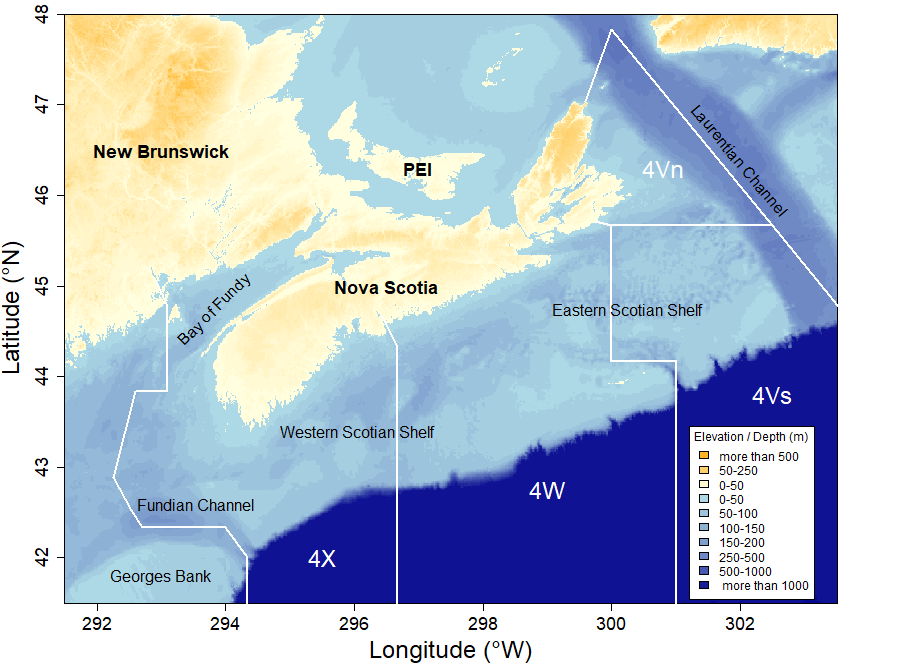
\includegraphics[width=6in]{./figures/annotated-map-NAFO}}{Figure \ref{fig:map1}} 

}

\caption{Map of the Scotian Shelf and Bay of Fundy.}\label{fig:map1}
\end{figure}
\hypertarget{sampling-design}{%
\subsection{Sampling Design}\label{sampling-design}}

The summer survey covers divisions 4V, 4W and 4X of the Northwest Atlantic Fisheries Organization (NAFO) which includes the Scotian Shelf and the Bay of Fundy. The eastern limit of the survey is the Laurentian Channel and the western limit is the Fundian Channel (Figure~\ref{fig:map1}).

The survey follows a stratified random design (Doubleday and Rivard \protect\hyperlink{ref-DoubledayRivard1981}{1981}; Lohr \protect\hyperlink{ref-Lohr1999}{1999}) (Figure~\ref{fig:map2}). The number of tows conducted in each stratum is approximately proportional to its surface area.


\begin{figure}[htb]

{\centering \pdftooltip{
\includegraphics[width=6in]{./figures/SUMMER-strata-map}}{Figure \ref{fig:map2}} 

}

\caption{Map of the Summer survey strata.}\label{fig:map2}
\end{figure}
The basic sampling unit of the survey is a 30-minute fishing tow conducted at a speed of 3.5 knots. This yields a distance towed of 1.75 nautical miles.

After each tow the catch is sorted by species and weighed. Each fish caught is then measured, and further sampling of individual fish weight, maturity status and age are performed for different length classes. When catches exceed 300 individuals, a random sub-sample is used to obtain the length and weight measurements.

The location of representative tows appears in Figure~\ref{fig:map3}.


\begin{figure}[htb]

{\centering \pdftooltip{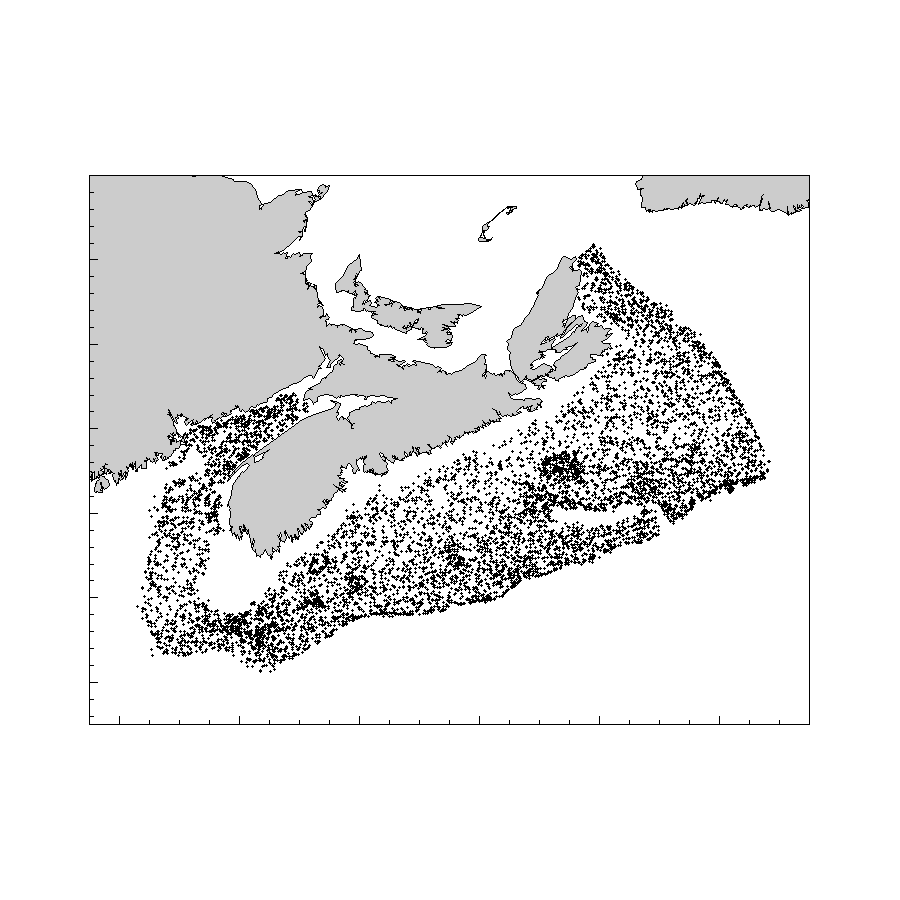
\includegraphics[width=6in]{./figures/SUMMER-tows-map}}{Figure \ref{fig:map3}} 

}

\caption{Map of the Summer survey tows.}\label{fig:map3}
\end{figure}
\hypertarget{taxo}{%
\subsection{Taxonomic Levels}\label{taxo}}

Fish species caught during the surveys are identified by trained scientific personnel and their scientific name is determined. An internal species code used in the relational database is reported for each species (Losier and Waite \protect\hyperlink{ref-LosierWaite1989}{1989}).

By its nature as a bottom trawl, the fishing gear used in the survey catches certain species better than others. To ensure that meaningful ecological information can be extracted from catch samples, we report the catch records for the subset of species that are caught reliably by the gear. To appear in this atlas, a species must have had a minimum of 10 observations over the duration of the survey activities. While both catch abundance and weight are recorded, the weight of species that appear at low abundances is often recorded as zero in the earlier parts of the survey when scales of appropriate precision were not available.

We divided the species caught into five categories based on 1) their taxonomic classification, 2) the number of recorded observations, and 3) their period of valid identification (Table~\ref{tab:taxocat}). Category ''LF'', for ''long frequent'', was assigned to species that have more than 1000 records since 1970 and have been consistently identified since the onset of the survey. Category ''LI'', for ''long intermediate'', was assigned to species that had between 1000 and 200 catch records. Rare and elusive species (those with less than 200 catch records over the duration of the survey) are also reported but to a lower level of analytical details (Category ''LR'', for ''long rare''). Category ''SF'', for ''short frequent'', was assigned to invertebrate species that were consistently sampled only since 1999 (Tremblay M. J. \protect\hyperlink{ref-Tremblayetal:2007}{2007}). And category ''SR'', for ''short rare'' for invertebrate species consistently sampled only since 1999 and with less than 200 catch records
\begin{table}
\begin{tabular}{p{0.1\textwidth}p{0.2\textwidth}p{0.7\textwidth}}
\toprule
\bfseries{Category} & \bfseries{Name} & \bfseries{Description} \\
\midrule
L & \multicolumn{2}{l}{long - consistently identified since the onset of the survey in 1970}\\
\midrule
LF & long frequent & species that have more than 1000 catch records \\

LI & long intermediate & species that had between 1000 and 200 catch records\\

LR & long rare & species with less than 200 catch records\\
\midrule
S & \multicolumn{2}{l}{short - invertebrate species that were consistently sampled only since 1999}\\
\midrule
SF & short frequent & species with more than 200 catch records \\

SR & short rare & species with less than 200 catch records\\
\bottomrule
\end{tabular}
\caption{Taxonomic levels}
\label{tab:taxocat}
\end{table}
The list of taxa covered in this document is presented in phylogenetic order (Nelson J. S. et al. \protect\hyperlink{ref-Nelsonetal:2004}{2004}) in Table~\ref{tab:tabspecies}. To ensure concordance with authoritative taxonomic information, the AphiaID from the World Register of Marine Species is also provided in Table~\ref{tab:tabspecies} (Appeltans et al. \protect\hyperlink{ref-WoRMS}{2012}).



\begingroup\fontsize{9}{11}\selectfont
\begin{landscape}
\begin{longtable}[t]{ccc>{\centering\arraybackslash}p{3cm}>{\centering\arraybackslash}p{3cm}>{\centering\arraybackslash}p{3cm}>{}c>{}ccc}
\caption{\label{tab:tabspecies}List of species included in the Atlas. The species reported here are listed in phylogenetic order as per Page L. M. et al. (\protect\hyperlink{ref-page:etal:7thedition}{2013}). For each taxonomic order and class, each species is listed in the table, its taxonomic family and scientific name is provided, along with its French and English common names, the species code used in the survey database, its AphiaID and a link to the World Registry of Marine Species, its number of catch records in the survey database and its classification category as defined in section~\ref{taxo}.}\\
\toprule
 &  & Family & Scientific name & English name & French name & Species code & AphiaID & Num. records & Category\\
\midrule
\endfirsthead
\caption*{}\\
\toprule
 &  & Family & Scientific name & English name & French name & Species code & AphiaID & Num. records & Category\\
\midrule
\endhead

\endfoot
\bottomrule
\endlastfoot
\addlinespace[0.3em]
\multicolumn{10}{l}{\textbf{Myxini}}\\
\addlinespace[0.3em]
\multicolumn{10}{l}{\textit{Myxiniformes}}\\
\hspace{1em}\hspace{1em} &  & Myxinidae & \em{Myxine glutinosa} & Atlantic hagfish & Myxine du nord & \href{#sec:241}{241} & \href{http://www.marinespecies.org/aphia.php?p=taxdetails&id=101170}{101170} & 804 & I\\
\cmidrule{1-10}\pagebreak[0]
\addlinespace[0.3em]
\multicolumn{10}{l}{\textbf{Petromyzonti}}\\
\addlinespace[0.3em]
\multicolumn{10}{l}{\textit{Petromyzontiformes}}\\
\hspace{1em}\hspace{1em} &  & Petromyzontidae & \em{Petromyzon marinus} & Sea lamprey & Lamproie marine & \href{#sec:240}{240} & \href{http://www.marinespecies.org/aphia.php?p=taxdetails&id=101174}{101174} & 16 & LR\\
\cmidrule{1-10}\pagebreak[0]
\addlinespace[0.3em]
\multicolumn{10}{l}{\textbf{Actinopterygii}}\\
\addlinespace[0.3em]
\multicolumn{10}{l}{\textit{Gadiformes}}\\
\hspace{1em}\hspace{1em} &  & Gadidae & \em{Gadus morhua} & Atlantic cod & Morue franche & \href{#sec:10}{10} & \href{http://www.marinespecies.org/aphia.php?p=taxdetails&id=126436}{126436} & 5451 & L\\
\cmidrule{4-10}\nopagebreak
\hspace{1em}\hspace{1em} &  &  & \em{Melanogrammus aeglefinus} & Haddock & Aiglefin & \href{#sec:11}{11} & \href{http://www.marinespecies.org/aphia.php?p=taxdetails&id=126437}{126437} & 5827 & L\\
\cmidrule{3-10}\nopagebreak
\hspace{1em}\hspace{1em} &  & Phycidae & \em{Urophycis tenuis} & White hake & Merluche blanche & \href{#sec:12}{12} & \href{http://www.marinespecies.org/aphia.php?p=taxdetails&id=126504}{126504} & 3524 & L\\
\cmidrule{4-10}\nopagebreak
\hspace{1em}\hspace{1em} &  &  & \em{Urophycis chuss} & Red hake & Merluche écureuil & \href{#sec:13}{13} & \href{http://www.marinespecies.org/aphia.php?p=taxdetails&id=126503}{126503} & 2195 & L\\
\cmidrule{3-10}\nopagebreak
\hspace{1em}\hspace{1em} &  & Merlucciidae & \em{Merluccius bilinearis} & Silver hake & Merlu argenté & \href{#sec:14}{14} & \href{http://www.marinespecies.org/aphia.php?p=taxdetails&id=158962}{158962} & 4936 & L\\
\cmidrule{3-10}\nopagebreak
\hspace{1em}\hspace{1em} &  & Lotidae & \em{Brosme brosme} & Cusk & Brosme & \href{#sec:15}{15} & \href{http://www.marinespecies.org/aphia.php?p=taxdetails&id=126447}{126447} & 688 & I\\
\cmidrule{3-10}\nopagebreak
\hspace{1em}\hspace{1em} &  & Gadidae & \em{Pollachius virens} & Pollock & Goberge & \href{#sec:16}{16} & \href{http://www.marinespecies.org/aphia.php?p=taxdetails&id=126441}{126441} & 2787 & L\\
\cmidrule{4-10}\nopagebreak
\hspace{1em}\hspace{1em} &  &  & \em{Microgadus tomcod} & Atlantic tomcod & Poulamon atlantique & \href{#sec:17}{17} & \href{http://www.marinespecies.org/aphia.php?p=taxdetails&id=158928}{158928} & 44 & LR\\
\cmidrule{3-10}\nopagebreak
\hspace{1em}\hspace{1em} &  & Merlucciidae & \em{Merluccius albidus} & Offshore silver hake & Merlu argenté du large & \href{#sec:19}{19} & \href{http://www.marinespecies.org/aphia.php?p=taxdetails&id=158748}{158748} & 161 & LR\\
\cmidrule{2-10}\nopagebreak
\addlinespace[0.3em]
\multicolumn{10}{l}{\textit{Scorpaeniformes}}\\
\hspace{1em}\hspace{1em} &  & Sebastidae & \em{Sebastes} & Atlantic redfishes & Sébastes de l'Atlantique & \href{#sec:23}{23} & \href{http://www.marinespecies.org/aphia.php?p=taxdetails&id=126175}{126175} & 4152 & L\\
\cmidrule{2-10}\nopagebreak
\addlinespace[0.3em]
\multicolumn{10}{l}{\textit{Pleuronectiformes}}\\
\hspace{1em}\hspace{1em} &  & Pleuronectidae & \em{Hippoglossus hippoglossus} & Atlantic halibut & Flétan de l'Atlantique & \href{#sec:30}{30} & \href{http://www.marinespecies.org/aphia.php?p=taxdetails&id=127138}{127138} & 1634 & L\\
\cmidrule{4-10}\nopagebreak
\hspace{1em}\hspace{1em} &  &  & \em{Reinhardtius hippoglossoides} & Greenland halibut & Flétan noir & \href{#sec:31}{31} & \href{http://www.marinespecies.org/aphia.php?p=taxdetails&id=127144}{127144} & 736 & I\\
\cmidrule{4-10}\nopagebreak
\hspace{1em}\hspace{1em} &  &  & \em{Hippoglossoides platessoides} & American plaice & Plie canadienne & \href{#sec:40}{40} & \href{http://www.marinespecies.org/aphia.php?p=taxdetails&id=127137}{127137} & 6023 & L\\
\cmidrule{4-10}\nopagebreak
\hspace{1em}\hspace{1em} &  &  & \em{Glyptocephalus cynoglossus} & Witch flounder & Plie grise & \href{#sec:41}{41} & \href{http://www.marinespecies.org/aphia.php?p=taxdetails&id=127136}{127136} & 4301 & L\\
\cmidrule{4-10}\nopagebreak
\hspace{1em}\hspace{1em} &  &  & \em{Limanda ferruginea} & Yellowtail flounder & Limande à queue jaune & \href{#sec:42}{42} & \href{http://www.marinespecies.org/aphia.php?p=taxdetails&id=158879}{158879} & 3233 & L\\
\cmidrule{4-10}\nopagebreak
\hspace{1em}\hspace{1em} &  &  & \em{Pseudopleuronectes americanus} & Winter flounder & Limande-plie rouge & \href{#sec:43}{43} & \href{http://www.marinespecies.org/aphia.php?p=taxdetails&id=158885}{158885} & 1632 & L\\
\cmidrule{3-10}\nopagebreak
\hspace{1em}\hspace{1em} &  & Paralichthyidae & \em{Citharichthys arctifrons} & Gulf Stream flounder & Plie du Gulf Stream & \href{#sec:44}{44} & \href{http://www.marinespecies.org/aphia.php?p=taxdetails&id=158791}{158791} & 382 & I\\
\cmidrule{2-10}\nopagebreak
\addlinespace[0.3em]
\multicolumn{10}{l}{\textit{Perciformes}}\\
\hspace{1em}\hspace{1em} &  & Anarhichadidae & \em{Anarhichas lupus} & Atlantic wolffish & Loup atlantique & \href{#sec:50}{50} & \href{http://www.marinespecies.org/aphia.php?p=taxdetails&id=126758}{126758} & 1572 & L\\
\cmidrule{4-10}\nopagebreak
\hspace{1em}\hspace{1em} &  &  & \em{Anarhichas minor} & Spotted wolffish & Loup tacheté & \href{#sec:51}{51} & \href{http://www.marinespecies.org/aphia.php?p=taxdetails&id=126759}{126759} & 20 & LR\\
\cmidrule{4-10}\nopagebreak
\hspace{1em}\hspace{1em} &  &  & \em{Anarhichas denticulatus} & Northern wolffish & Loup à tête large & \href{#sec:52}{52} & \href{http://www.marinespecies.org/aphia.php?p=taxdetails&id=126757}{126757} & 17 & LR\\
\cmidrule{2-10}\nopagebreak
\addlinespace[0.3em]
\multicolumn{10}{l}{\textit{Clupeiformes}}\\
\hspace{1em}\hspace{1em} &  & Clupeidae & \em{Clupea harengus} & Atlantic herring & Hareng de l'Atlantique & \href{#sec:60}{60} & \href{http://www.marinespecies.org/aphia.php?p=taxdetails&id=126417}{126417} & 3487 & L\\
\cmidrule{4-10}\nopagebreak
\hspace{1em}\hspace{1em} &  &  & \em{Alosa sapidissima} & American shad & Alose savoureuse & \href{#sec:61}{61} & \href{http://www.marinespecies.org/aphia.php?p=taxdetails&id=158670}{158670} & 468 & I\\
\cmidrule{4-10}\nopagebreak
\hspace{1em}\hspace{1em} &  &  & \em{Alosa pseudoharengus} & Alewife & Gaspareau & \href{#sec:62}{62} & \href{http://www.marinespecies.org/aphia.php?p=taxdetails&id=158669}{158669} & 977 & I\\
\cmidrule{2-10}\nopagebreak
\addlinespace[0.3em]
\multicolumn{10}{l}{\textit{Osmeriformes}}\\
\hspace{1em}\hspace{1em} &  & Osmeridae & \em{Osmerus mordax} & Rainbow smelt & Éperlan arc-en-ciel & \href{#sec:63}{63} & \href{http://www.marinespecies.org/aphia.php?p=taxdetails&id=126737}{126737} & 59 & LR\\
\cmidrule{4-10}\nopagebreak
\hspace{1em}\hspace{1em} &  &  & \em{Mallotus villosus} & Capelin & Capelan & \href{#sec:64}{64} & \href{http://www.marinespecies.org/aphia.php?p=taxdetails&id=126735}{126735} & 540 & I\\
\cmidrule{2-10}\nopagebreak
\addlinespace[0.3em]
\multicolumn{10}{l}{\textit{Perciformes}}\\
\hspace{1em}\hspace{1em} &  & Scombridae & \em{Scomber scombrus} & Atlantic mackerel & Maquereau commun & \href{#sec:70}{70} & \href{http://www.marinespecies.org/aphia.php?p=taxdetails&id=127023}{127023} & 696 & I\\
\cmidrule{2-10}\nopagebreak
\addlinespace[0.3em]
\multicolumn{10}{l}{\textit{Gadiformes}}\\
\hspace{1em}\hspace{1em} &  & Phycidae & \em{Phycis chesteri} & Longfin hake & Merluche à longues nageoires & \href{#sec:112}{112} & \href{http://www.marinespecies.org/aphia.php?p=taxdetails&id=158988}{158988} & 784 & I\\
\cmidrule{3-10}\nopagebreak
\hspace{1em}\hspace{1em} &  & Lotidae & \em{Enchelyopus cimbrius} & Fourbeard rockling & Motelle à quatre barbillons & \href{#sec:114}{114} & \href{http://www.marinespecies.org/aphia.php?p=taxdetails&id=126450}{126450} & 693 & I\\
\cmidrule{2-10}\nopagebreak
\addlinespace[0.3em]
\multicolumn{10}{l}{\textit{Perciformes}}\\
\hspace{1em}\hspace{1em} &  & Labridae & \em{Tautogolabrus adspersus} & Cunner & Tanche-tautogue & \href{#sec:122}{122} & \href{http://www.marinespecies.org/aphia.php?p=taxdetails&id=159785}{159785} & 82 & LR\\
\cmidrule{2-10}\nopagebreak
\addlinespace[0.3em]
\multicolumn{10}{l}{\textit{Scorpaeniformes}}\\
\hspace{1em}\hspace{1em} &  & Sebastidae & \em{Helicolenus dactylopterus} & Blackbelly rosefish & Sébaste chèvre & \href{#sec:123}{123} & \href{http://www.marinespecies.org/aphia.php?p=taxdetails&id=127251}{127251} & 610 & I\\
\cmidrule{2-10}\nopagebreak
\addlinespace[0.3em]
\multicolumn{10}{l}{\textit{Pleuronectiformes}}\\
\hspace{1em}\hspace{1em} &  & Paralichthyidae & \em{Hippoglossina oblonga} & Fourspot flounder & Cardeau à quatre ocelles & \href{#sec:142}{142} & \href{http://www.marinespecies.org/aphia.php?p=taxdetails&id=158833}{158833} & 76 & LR\\
\cmidrule{3-10}\nopagebreak
\hspace{1em}\hspace{1em} &  & Scophthalmidae & \em{Scophthalmus aquosus} & Windowpane flounder & Turbot de sable & \href{#sec:143}{143} & \href{http://www.marinespecies.org/aphia.php?p=taxdetails&id=158907}{158907} & 115 & LR\\
\cmidrule{2-10}\nopagebreak
\addlinespace[0.3em]
\multicolumn{10}{l}{\textit{Aulopiformes}}\\
\hspace{1em}\hspace{1em} &  & Chlorophthalmidae & \em{Parasudis truculenta} & Longnose greeneye & Oeil-vert à long nez & \href{#sec:149}{149} & \href{http://www.marinespecies.org/aphia.php?p=taxdetails&id=158868}{158868} & 45 & LR\\
\cmidrule{2-10}\nopagebreak
\addlinespace[0.3em]
\multicolumn{10}{l}{\textit{Myctophiformes}}\\
\hspace{1em}\hspace{1em} &  & Myctophidae & \em{Myctophidae} & Lanternfishes & Poissons-lanternes & \href{#sec:150}{150} & \href{http://www.marinespecies.org/aphia.php?p=taxdetails&id=125498}{125498} & 160 & LR\\
\cmidrule{2-10}\nopagebreak
\addlinespace[0.3em]
\multicolumn{10}{l}{\textit{Aulopiformes}}\\
\hspace{1em}\hspace{1em} &  & Chlorophthalmidae & \em{Chlorophthalmus agassizi} & Shortnose greeneye & Éperlan du large & \href{#sec:156}{156} & \href{http://www.marinespecies.org/aphia.php?p=taxdetails&id=126336}{126336} & 78 & LR\\
\cmidrule{2-10}\nopagebreak
\addlinespace[0.3em]
\multicolumn{10}{l}{\textit{Stomiiformes}}\\
\hspace{1em}\hspace{1em} &  & Sternoptychidae & \em{Maurolicus muelleri} & Silvery lightfish & Brossé améthyste & \href{#sec:158}{158} & \href{http://www.marinespecies.org/aphia.php?p=taxdetails&id=127312}{127312} & 52 & LR\\
\cmidrule{3-10}\nopagebreak
\hspace{1em}\hspace{1em} &  & Stomiidae & \em{Stomias boa} & Boa dragonfish & Dragon-boa & \href{#sec:159}{159} & \href{http://www.marinespecies.org/aphia.php?p=taxdetails&id=127374}{127374} & 20 & LR\\
\cmidrule{2-10}\nopagebreak
\addlinespace[0.3em]
\multicolumn{10}{l}{\textit{Argentiniformes}}\\
\hspace{1em}\hspace{1em} &  & Argentinidae & \em{Argentina silus} & Greater argentine & Grande argentine & \href{#sec:160}{160} & \href{http://www.marinespecies.org/aphia.php?p=taxdetails&id=126715}{126715} & 963 & I\\
\cmidrule{2-10}\nopagebreak
\addlinespace[0.3em]
\multicolumn{10}{l}{\textit{Scorpaeniformes}}\\
\hspace{1em}\hspace{1em} &  & Cottidae & \em{Myoxocephalus octodecemspinosus} & Longhorn sculpin & Chaboisseau à dix-huit épines & \href{#sec:300}{300} & \href{http://www.marinespecies.org/aphia.php?p=taxdetails&id=159520}{159520} & 3292 & L\\
\cmidrule{4-10}\nopagebreak
\hspace{1em}\hspace{1em} &  &  & \em{Myoxocephalus scorpius} & Shorthorn sculpin & Chaboisseau à épines courtes & \href{#sec:301}{301} & \href{http://www.marinespecies.org/aphia.php?p=taxdetails&id=127203}{127203} & 131 & LR\\
\cmidrule{4-10}\nopagebreak
\hspace{1em}\hspace{1em} &  &  & \em{Myoxocephalus aenaeus} & Grubby & Chaboisseau bronzé & \href{#sec:303}{303} & \href{http://www.marinespecies.org/aphia.php?p=taxdetails&id=159519}{159519} & 40 & LR\\
\cmidrule{4-10}\nopagebreak
\hspace{1em}\hspace{1em} &  &  & \em{Triglops murrayi} & Moustache sculpin & Faux-trigle armé & \href{#sec:304}{304} & \href{http://www.marinespecies.org/aphia.php?p=taxdetails&id=127205}{127205} & 1182 & L\\
\cmidrule{4-10}\nopagebreak
\hspace{1em}\hspace{1em} &  &  & \em{Artediellus uncinatus} & Arctic hookear sculpin & Hameçon neigeux & \href{#sec:306}{306} & \href{http://www.marinespecies.org/aphia.php?p=taxdetails&id=127195}{127195} & 306 & I\\
\cmidrule{3-10}\nopagebreak
\hspace{1em}\hspace{1em} &  & Psychrolutidae & \em{Cottunculus microps} & Polar sculpin & Cotte polaire & \href{#sec:307}{307} & \href{http://www.marinespecies.org/aphia.php?p=taxdetails&id=127235}{127235} & 29 & LR\\
\cmidrule{3-10}\nopagebreak
\hspace{1em}\hspace{1em} &  & Cottidae & \em{Icelus spatula} & Spatulate sculpin & Icèle spatulée & \href{#sec:314}{314} & \href{http://www.marinespecies.org/aphia.php?p=taxdetails&id=127200}{127200} & 40 & LR\\
\cmidrule{3-10}\nopagebreak
\hspace{1em}\hspace{1em} &  & Hemitripteridae & \em{Hemitripterus americanus} & Sea raven & Hémitriptère atlantique & \href{#sec:320}{320} & \href{http://www.marinespecies.org/aphia.php?p=taxdetails&id=159518}{159518} & 2126 & L\\
\cmidrule{3-10}\nopagebreak
\hspace{1em}\hspace{1em} &  & Agonidae & \em{Aspidophoroides monopterygius} & Alligatorfish & Poisson-alligator atlantique & \href{#sec:340}{340} & \href{http://www.marinespecies.org/aphia.php?p=taxdetails&id=159459}{159459} & 1029 & L\\
\cmidrule{4-10}\nopagebreak
\hspace{1em}\hspace{1em} &  &  & \em{Ulcina olrikii} & Arctic alligatorfish & Poisson-alligator arctique & \href{#sec:341}{341} & \href{http://www.marinespecies.org/aphia.php?p=taxdetails&id=274356}{274356} & 13 & LR\\
\cmidrule{4-10}\nopagebreak
\hspace{1em}\hspace{1em} &  &  & \em{Leptagonus decagonus} & Atlantic poacher & Agone atlantique & \href{#sec:350}{350} & \href{http://www.marinespecies.org/aphia.php?p=taxdetails&id=127191}{127191} & 266 & I\\
\cmidrule{4-10}\nopagebreak
\hspace{1em}\hspace{1em} &  &  & \em{Agonidae} & Alligatorfishes & Poissons-alligator & \href{#sec:351}{351} & \href{http://www.marinespecies.org/aphia.php?p=taxdetails&id=125588}{125588} & 43 & LR\\
\cmidrule{2-10}\nopagebreak
\addlinespace[0.3em]
\multicolumn{10}{l}{\textit{Lophiiformes}}\\
\hspace{1em}\hspace{1em} &  & Lophiidae & \em{Lophius americanus} & Monkfish & Baudroie d'Amérique & \href{#sec:400}{400} & \href{http://www.marinespecies.org/aphia.php?p=taxdetails&id=159184}{159184} & 1970 & L\\
\cmidrule{2-10}\nopagebreak
\addlinespace[0.3em]
\multicolumn{10}{l}{\textit{Gadiformes}}\\
\hspace{1em}\hspace{1em} &  & Macrouridae & \em{Nezumia bairdii} & Marlin-spike grenadier & Grenadier du Grand Banc & \href{#sec:410}{410} & \href{http://www.marinespecies.org/aphia.php?p=taxdetails&id=183289}{183289} & 529 & I\\
\cmidrule{4-10}\nopagebreak
\hspace{1em}\hspace{1em} &  &  & \em{Trachyrincus murrayi} & Roughnose grenadier & Grenadier-scie & \href{#sec:412}{412} & \href{http://www.marinespecies.org/aphia.php?p=taxdetails&id=126481}{126481} & 18 & LR\\
\cmidrule{4-10}\nopagebreak
\hspace{1em}\hspace{1em} &  &  & \em{Coryphaenoides rupestris} & Roundnose grenadier & Grenadier de roche & \href{#sec:414}{414} & \href{http://www.marinespecies.org/aphia.php?p=taxdetails&id=158960}{158960} & 17 & LR\\
\cmidrule{2-10}\nopagebreak
\addlinespace[0.3em]
\multicolumn{10}{l}{\textit{Scorpaeniformes}}\\
\hspace{1em}\hspace{1em} &  & Cyclopteridae & \em{Cyclopterus lumpus} & Lumpfish & Lompe & \href{#sec:501}{501} & \href{http://www.marinespecies.org/aphia.php?p=taxdetails&id=127214}{127214} & 216 & I\\
\cmidrule{4-10}\nopagebreak
\hspace{1em}\hspace{1em} &  &  & \em{Eumicrotremus spinosus} & Atlantic spiny lumpsucker & Petite poule de mer atlantique & \href{#sec:502}{502} & \href{http://www.marinespecies.org/aphia.php?p=taxdetails&id=127217}{127217} & 226 & I\\
\cmidrule{3-10}\nopagebreak
\hspace{1em}\hspace{1em} &  & Liparidae & \em{Liparis atlanticus} & Atlantic seasnail & Limace atlantique & \href{#sec:503}{503} & \href{http://www.marinespecies.org/aphia.php?p=taxdetails&id=159524}{159524} & 34 & LR\\
\cmidrule{4-10}\nopagebreak
\hspace{1em}\hspace{1em} &  &  & \em{Liparis fabricii} & Gelatinous snailfish & Limace gélatineuse & \href{#sec:505}{505} & \href{http://www.marinespecies.org/aphia.php?p=taxdetails&id=127218}{127218} & 27 & LR\\
\cmidrule{4-10}\nopagebreak
\hspace{1em}\hspace{1em} &  &  & \em{Liparis gibbus} & Variegated snailfish & Limace marbée & \href{#sec:512}{512} & \href{http://www.marinespecies.org/aphia.php?p=taxdetails&id=159526}{159526} & 41 & LR\\
\cmidrule{4-10}\nopagebreak
\hspace{1em}\hspace{1em} &  &  & \em{Careproctus reinhardti} & Sea tadpole & Petite limace de mer & \href{#sec:520}{520} & \href{http://www.marinespecies.org/aphia.php?p=taxdetails&id=127212}{127212} & 18 & LR\\
\cmidrule{2-10}\nopagebreak
\addlinespace[0.3em]
\multicolumn{10}{l}{\textit{Perciformes}}\\
\hspace{1em}\hspace{1em} &  & Zoarcidae & \em{Lycenchelys verrillii} & Wolf eelpout & Lycode à tête longue & \href{#sec:603}{603} & \href{http://www.marinespecies.org/aphia.php?p=taxdetails&id=159258}{159258} & 40 & LR\\
\cmidrule{2-10}\nopagebreak
\addlinespace[0.3em]
\multicolumn{10}{l}{\textit{Anguilliformes}}\\
\hspace{1em}\hspace{1em} &  & Nemichthyidae & \em{Nemichthys scolopaceus} & Slender snipe eel & Avocette ruban & \href{#sec:604}{604} & \href{http://www.marinespecies.org/aphia.php?p=taxdetails&id=126306}{126306} & 28 & LR\\
\cmidrule{2-10}\nopagebreak
\addlinespace[0.3em]
\multicolumn{10}{l}{\textit{Perciformes}}\\
\hspace{1em}\hspace{1em} &  & Ammodytidae & \em{Ammodytes dubius} & Sand lance & Lançon & \href{#sec:610}{610} & \href{http://www.marinespecies.org/aphia.php?p=taxdetails&id=151520}{151520} & 1283 & I\\
\cmidrule{3-10}\nopagebreak
\hspace{1em}\hspace{1em} &  & Zoarcidae & \em{Lycodes terraenovae} & Newfoundland eelpout & Lycode du Labrador & \href{#sec:619}{619} & \href{http://www.marinespecies.org/aphia.php?p=taxdetails&id=127117}{127117} & 64 & LR\\
\cmidrule{4-10}\nopagebreak
\hspace{1em}\hspace{1em} &  &  & \em{Lycodes lavalaei} & Newfoundland eelpout & Lycode du Labrador & \href{#sec:620}{620} & \href{http://www.marinespecies.org/aphia.php?p=taxdetails&id=127107}{127107} & 72 & LR\\
\cmidrule{3-10}\nopagebreak
\hspace{1em}\hspace{1em} &  & Pholidae & \em{Pholis gunnellus} & Rock gunnel & Sigouine de roche & \href{#sec:621}{621} & \href{http://www.marinespecies.org/aphia.php?p=taxdetails&id=126996}{126996} & 21 & LR\\
\cmidrule{3-10}\nopagebreak
\hspace{1em}\hspace{1em} &  & Stichaeidae & \em{Lumpenus lampretaeformis} & Snakeblenny & Lompénie-serpent & \href{#sec:622}{622} & \href{http://www.marinespecies.org/aphia.php?p=taxdetails&id=154675}{154675} & 423 & I\\
\cmidrule{4-10}\nopagebreak
\hspace{1em}\hspace{1em} &  &  & \em{Leptoclinus maculatus} & Daubed shanny & Lompénie tachetée & \href{#sec:623}{623} & \href{http://www.marinespecies.org/aphia.php?p=taxdetails&id=127072}{127072} & 443 & I\\
\cmidrule{4-10}\nopagebreak
\hspace{1em}\hspace{1em} &  &  & \em{Ulvaria subbifurcata} & Radiated shanny & Ulvaire deux-lignes & \href{#sec:625}{625} & \href{http://www.marinespecies.org/aphia.php?p=taxdetails&id=159821}{159821} & 145 & LR\\
\cmidrule{4-10}\nopagebreak
\hspace{1em}\hspace{1em} &  &  & \em{Eumesogrammus praecisus} & Fourline snakeblenny & Quatre-lignes atlantique & \href{#sec:626}{626} & \href{http://www.marinespecies.org/aphia.php?p=taxdetails&id=159817}{159817} & 40 & LR\\
\cmidrule{3-10}\nopagebreak
\hspace{1em}\hspace{1em} &  & Cryptacanthodidae & \em{Cryptacanthodes maculatus} & Wrymouth & Terrassier tacheté & \href{#sec:630}{630} & \href{http://www.marinespecies.org/aphia.php?p=taxdetails&id=159675}{159675} & 120 & LR\\
\cmidrule{3-10}\nopagebreak
\hspace{1em}\hspace{1em} &  & Callionymidae & \em{Foetorepus agassizii} & Spotfin dragonet & Dragonnet tacheté & \href{#sec:637}{637} & \href{http://www.marinespecies.org/aphia.php?p=taxdetails&id=276339}{276339} & 20 & LR\\
\cmidrule{3-10}\nopagebreak
\hspace{1em}\hspace{1em} &  & Zoarcidae & \em{Zoarces americanus} & Ocean pout & Loquette d'Amérique & \href{#sec:640}{640} & \href{http://www.marinespecies.org/aphia.php?p=taxdetails&id=159267}{159267} & 1478 & L\\
\cmidrule{4-10}\nopagebreak
\hspace{1em}\hspace{1em} &  &  & \em{Lycodes reticulatus} & Arctic eelpout & Lycode arctique & \href{#sec:641}{641} & \href{http://www.marinespecies.org/aphia.php?p=taxdetails&id=127112}{127112} & 70 & LR\\
\cmidrule{4-10}\nopagebreak
\hspace{1em}\hspace{1em} &  &  & \em{Melanostigma atlanticum} & Atlantic soft pout & Molasse atlantique & \href{#sec:646}{646} & \href{http://www.marinespecies.org/aphia.php?p=taxdetails&id=127120}{127120} & 43 & LR\\
\cmidrule{4-10}\nopagebreak
\hspace{1em}\hspace{1em} &  &  & \em{Lycodes vahlii} & Vahl's eelpout & Lycode à carreaux & \href{#sec:647}{647} & \href{http://www.marinespecies.org/aphia.php?p=taxdetails&id=127118}{127118} & 565 & I\\
\cmidrule{3-10}\nopagebreak
\hspace{1em}\hspace{1em} &  & Stromateidae & \em{Peprilus triacanthus} & Atlantic butterfish & Stromaté fossette & \href{#sec:701}{701} & \href{http://www.marinespecies.org/aphia.php?p=taxdetails&id=159828}{159828} & 487 & I\\
\cmidrule{2-10}\nopagebreak
\addlinespace[0.3em]
\multicolumn{10}{l}{\textit{Zeiformes}}\\
\hspace{1em}\hspace{1em} &  & Zeidae & \em{Zenopsis conchifer} & Silvery John dory & Saint Pierre argenté & \href{#sec:704}{704} & \href{http://www.marinespecies.org/aphia.php?p=taxdetails&id=127426}{127426} & 39 & LR\\
\cmidrule{2-10}\nopagebreak
\addlinespace[0.3em]
\multicolumn{10}{l}{\textit{Aulopiformes}}\\
\hspace{1em}\hspace{1em} &  & Paralepididae & \em{Arctozenus risso} & White barracudina & Lussion blanc & \href{#sec:712}{712} & \href{http://www.marinespecies.org/aphia.php?p=taxdetails&id=126352}{126352} & 196 & LR\\
\cmidrule{2-10}\nopagebreak
\addlinespace[0.3em]
\multicolumn{10}{l}{\textit{Beloniformes}}\\
\hspace{1em}\hspace{1em} &  & Scomberesocidae & \em{Scomberesox saurus} & Atlantic saury & Balaou atlantique & \href{#sec:720}{720} & \href{http://www.marinespecies.org/aphia.php?p=taxdetails&id=126392}{126392} & 37 & LR\\
\cmidrule{2-10}\nopagebreak
\addlinespace[0.3em]
\multicolumn{10}{l}{\textit{Stomiiformes}}\\
\hspace{1em}\hspace{1em} &  & Sternoptychidae & \em{Sternoptychidae} & Hatchetfishes & Haches d'argent & \href{#sec:741}{741} & \href{http://www.marinespecies.org/aphia.php?p=taxdetails&id=125603}{125603} & 21 & LR\\
\cmidrule{2-10}\nopagebreak
\addlinespace[0.3em]
\multicolumn{10}{l}{\textit{Lophiiformes}}\\
\hspace{1em}\hspace{1em} &  & Ogcocephalidae & \em{Dibranchus atlanticus} & Atlantic batfish & Malthe atlantique & \href{#sec:742}{742} & \href{http://www.marinespecies.org/aphia.php?p=taxdetails&id=126558}{126558} & 18 & LR\\
\cmidrule{2-10}\nopagebreak
\addlinespace[0.3em]
\multicolumn{10}{l}{\textit{Pleuronectiformes}}\\
\hspace{1em}\hspace{1em} &  & Cynoglossidae & \em{Symphurus diomedeanus} & Spottedfin tonguefish & Langue fil noir & \href{#sec:816}{816} & \href{http://www.marinespecies.org/aphia.php?p=taxdetails&id=159358}{159358} & 24 & LR\\
\cmidrule{2-10}\nopagebreak
\addlinespace[0.3em]
\multicolumn{10}{l}{\textit{Scorpaeniformes}}\\
\hspace{1em}\hspace{1em} &  & Cottidae & \em{Artediellus atlanticus} & Atlantic hookear sculpin & Hameçon atlantique & \href{#sec:880}{880} & \href{http://www.marinespecies.org/aphia.php?p=taxdetails&id=127193}{127193} & 258 & I\\
\cmidrule{1-10}\pagebreak[0]
\addlinespace[0.3em]
\multicolumn{10}{l}{\textbf{Elasmobranchii}}\\
\addlinespace[0.3em]
\multicolumn{10}{l}{\textit{Rajiformes}}\\
\hspace{1em}\hspace{1em} &  & Rajidae & \em{Dipturus laevis} & Barndoor skate & Grande raie & \href{#sec:200}{200} & \href{http://www.marinespecies.org/aphia.php?p=taxdetails&id=158548}{158548} & 246 & I\\
\cmidrule{4-10}\nopagebreak
\hspace{1em}\hspace{1em} &  &  & \em{Amblyraja radiata} & Thorny skate & Raie épineuse & \href{#sec:201}{201} & \href{http://www.marinespecies.org/aphia.php?p=taxdetails&id=105865}{105865} & 3937 & L\\
\cmidrule{4-10}\nopagebreak
\hspace{1em}\hspace{1em} &  &  & \em{Malacoraja senta} & Smooth skate & Raie lisse & \href{#sec:202}{202} & \href{http://www.marinespecies.org/aphia.php?p=taxdetails&id=158554}{158554} & 1773 & L\\
\cmidrule{4-10}\nopagebreak
\hspace{1em}\hspace{1em} &  &  & \em{Leucoraja erinacea} & Little skate & Raie hérisson & \href{#sec:203}{203} & \href{http://www.marinespecies.org/aphia.php?p=taxdetails&id=158551}{158551} & 712 & I\\
\cmidrule{4-10}\nopagebreak
\hspace{1em}\hspace{1em} &  &  & \em{Leucoraja ocellata} & Winter skate & Raie tachetée & \href{#sec:204}{204} & \href{http://www.marinespecies.org/aphia.php?p=taxdetails&id=158553}{158553} & 1180 & L\\
\cmidrule{2-10}\nopagebreak
\addlinespace[0.3em]
\multicolumn{10}{l}{\textit{Squaliformes}}\\
\hspace{1em}\hspace{1em} &  & Squalidae & \em{Squalus acanthias} & Picked dogfish & Aiguillat commun & \href{#sec:220}{220} & \href{http://www.marinespecies.org/aphia.php?p=taxdetails&id=105923}{105923} & 1985 & L\\
\cmidrule{3-10}\nopagebreak
\hspace{1em}\hspace{1em} &  & Etmopteridae & \em{Centroscyllium fabricii} & Black dogfish & Aiguillat noir & \href{#sec:221}{221} & \href{http://www.marinespecies.org/aphia.php?p=taxdetails&id=105906}{105906} & 31 & LR\\
\cmidrule{1-10}\pagebreak[0]
\addlinespace[0.3em]
\multicolumn{10}{l}{\textbf{Cephalopoda}}\\
\addlinespace[0.3em]
\multicolumn{10}{l}{\textit{Oegopsida}}\\
\hspace{1em}\hspace{1em} &  & Ommastrephidae & \em{Illex illecebrosus} & Northern shortfin squid & Encornet rouge nordique & \href{#sec:4511}{4511} & \href{http://www.marinespecies.org/aphia.php?p=taxdetails&id=153087}{153087} & 4836 & L\\
\cmidrule{2-10}\nopagebreak
\addlinespace[0.3em]
\multicolumn{10}{l}{\textit{Myopsida}}\\
\hspace{1em}\hspace{1em} &  & Loliginidae & \em{Doryteuthis pealeii} & Longfin inshore squid & Calmar totam & \href{#sec:4512}{4512} & \href{http://www.marinespecies.org/aphia.php?p=taxdetails&id=574541}{574541} & 96 & LR\\
\cmidrule{1-10}\pagebreak[0]
\addlinespace[0.3em]
\multicolumn{10}{l}{\textbf{Malacostraca}}\\
\addlinespace[0.3em]
\multicolumn{10}{l}{\textit{Decapoda}}\\
\hspace{1em}\hspace{1em} &  & Pandalidae & \em{Pandalus borealis} & Northern prawn & Crevette nordique & \href{#sec:2211}{2211} & \href{http://www.marinespecies.org/aphia.php?p=taxdetails&id=107649}{107649} & 718 & S\\
\cmidrule{3-10}\nopagebreak
\hspace{1em}\hspace{1em} &  & Cancridae & \em{Cancer borealis} & Jonah crab & Tourteau jona & \href{#sec:2511}{2511} & \href{http://www.marinespecies.org/aphia.php?p=taxdetails&id=158056}{158056} & 1387 & S\\
\cmidrule{4-10}\nopagebreak
\hspace{1em}\hspace{1em} &  &  & \em{Cancer irroratus} & Atlantic rock crab & Tourteau poïnclos & \href{#sec:2513}{2513} & \href{http://www.marinespecies.org/aphia.php?p=taxdetails&id=158057}{158057} & 788 & S\\
\cmidrule{3-10}\nopagebreak
\hspace{1em}\hspace{1em} &  & Oregoniidae & \em{Hyas coarctatus} & Arctic lyre crab & Crabe Hyas coarctatus & \href{#sec:2521}{2521} & \href{http://www.marinespecies.org/aphia.php?p=taxdetails&id=107323}{107323} & 711 & S\\
\cmidrule{3-10}\nopagebreak
\hspace{1em}\hspace{1em} &  & Lithodidae & \em{Lithodes maja} & Atlantic king crab & Crabe épineux du nord & \href{#sec:2523}{2523} & \href{http://www.marinespecies.org/aphia.php?p=taxdetails&id=107205}{107205} & 531 & S\\
\cmidrule{3-10}\nopagebreak
\hspace{1em}\hspace{1em} &  & Oregoniidae & \em{Chionoecetes opilio} & Queen crab & Crabe des neiges & \href{#sec:2526}{2526} & \href{http://www.marinespecies.org/aphia.php?p=taxdetails&id=107315}{107315} & 1546 & S\\
\cmidrule{4-10}\nopagebreak
\hspace{1em}\hspace{1em} &  &  & \em{Hyas araneus} & Great spider crab & Crabe lyre araignée & \href{#sec:2527}{2527} & \href{http://www.marinespecies.org/aphia.php?p=taxdetails&id=107322}{107322} & 625 & S\\
\cmidrule{3-10}\nopagebreak
\hspace{1em}\hspace{1em} &  & Geryonidae & \em{Chaceon quinquedens} & Red deepsea crab & Crabe rouge & \href{#sec:2532}{2532} & \href{http://www.marinespecies.org/aphia.php?p=taxdetails&id=158407}{158407} & 33 & SR\\
\cmidrule{3-10}\nopagebreak
\hspace{1em}\hspace{1em} &  & Nephropidae & \em{Homarus americanus} & American lobster & Homard américain & \href{#sec:2550}{2550} & \href{http://www.marinespecies.org/aphia.php?p=taxdetails&id=156134}{156134} & 1623 & S\\*
\end{longtable}
\end{landscape}
\endgroup{}

\hypertarget{analyses}{%
\subsection{Analyses}\label{analyses}}

The Oracle relational database where all data are stored was accessible from the Bedford Institute of Oceanography in Dartmouth, Nova Scotia. Structured Query Language (SQL) is used to extract the data from the production server and to create the data products used in all subsequent analyses. Catch records classified as ''valid'' (i.e.~a representative tow without damage to the net) are used in the current analyses. To make the available samples comparable, catch number and weight for each species was standardized for the distance towed.

All data processing and analyses were conducted using the R software (R Core Team \protect\hyperlink{ref-R:2020}{2020}) using packages gstat (Pebesma \protect\hyperlink{ref-R:package:gstat}{2004}), PBSmapping (Schnute et al. \protect\hyperlink{ref-R:package:PBSmapping}{2019}), RODBC (Ripley and Lapsley \protect\hyperlink{ref-R:package:RODBC}{2019}), spatstat (Baddeley \protect\hyperlink{ref-R:package:spatstat}{2015}), maptools (Bivand and Lewin-Koh \protect\hyperlink{ref-R:package:maptools}{2020}), rgeos (Bivand and Rundel \protect\hyperlink{ref-R:package:rgeos}{2020}), classInt(Bivand \protect\hyperlink{ref-R:package:classInt}{2020}), RColorBrewer(Neuwirth \protect\hyperlink{ref-R:package:RColorBrewer}{2014}), MASS (Ripley et al. \protect\hyperlink{ref-R:package:MASS}{2020}), worms (Holstein \protect\hyperlink{ref-R:package:worms}{2018}), and tidyverse (Wickham \protect\hyperlink{ref-R:Tidyverse}{2019}). The present document is rendered as a Technical Report using the csasdown R package developed and maintained by Fisheries and Oceans Canada scientists (Anderson et al. \protect\hyperlink{ref-R:csasdown}{In press}).

\hypertarget{geographic-distribution-of-catches}{%
\subsubsection{Geographic distribution of catches}\label{geographic-distribution-of-catches}}

Spatial interpolation of catch biomass (kg/tow) or abundance (number/tow) was done using a weighting inversely proportional to the distance, using function ''idw'' of the spatstat R package (Baddeley \protect\hyperlink{ref-R:package:spatstat}{2015}).

\hypertarget{abundance-and-biomass-indices}{%
\subsubsection{Abundance and biomass indices}\label{abundance-and-biomass-indices}}

For each species, stratified random estimates of catch abundance and biomass (Smith \protect\hyperlink{ref-Smith:1996}{1996}) were computed for each year. Yearly estimates of the standard error were also computed.

\hypertarget{distribution-indices}{%
\subsubsection{Distribution indices}\label{distribution-indices}}

For each Category L, I and S fish species, the minimum area required to account for 75\% and 95\% of the total biomass or abundance were computed (D75\% and D95\%). These measures of distributions were computed for each year by using the Lorenz curve of mean stratum-level catch estimates and the area of occupied strata (Swain and Sinclair \protect\hyperlink{ref-Swain:Sinclair:1994:cjfas}{1994}; Swain and Morin \protect\hyperlink{ref-Swain:Morin:1996:cjfas}{1996}).

\hypertarget{length-frequencies}{%
\subsubsection{Length frequencies}\label{length-frequencies}}

The length frequency distribution of catch is tabulated for each seven-year period (1970-2009), and last ten-year period (2010-2020).

\hypertarget{length-weight-relationship-and-condition-factor}{%
\subsubsection{Length-weight relationship and condition factor}\label{length-weight-relationship-and-condition-factor}}

The relationship between the weight and the length of fish was estimated using the following non-linear isometric relationship:
\begin{eqnarray*}\label{eqLengthWeight}
W = \alpha L ^\beta  
\\
\end{eqnarray*}
where W is the total weight (g), L is the length (cm), and, \(\alpha\) and \(\beta\) are the parameters to be estimated.

Average fish condition (C) was computed as:
\begin{eqnarray*}\label{eqCondition}
C = \frac{W}{\alpha L ^\beta}  
\\
\end{eqnarray*}
\hypertarget{depth-temperature-and-salinity-distribution-of-catches}{%
\subsubsection{Depth, temperature and salinity distribution of catches}\label{depth-temperature-and-salinity-distribution-of-catches}}

For each category L species, We followed the methods developed by (Perry and Smith \protect\hyperlink{ref-Perry:Smith:1994:cjfas}{1994}) and generated cumulative frequency distributions of depth, temperature and salinity of survey catches.

\hypertarget{density-dependent-habitat-selection}{%
\subsubsection{Density-dependent habitat selection}\label{density-dependent-habitat-selection}}

We followed the methods of (Myers and Stokes \protect\hyperlink{ref-Myers:Stokes:1989}{1989}) to evaluate how fish abundance in each stratum varied with overall temporal fluctuations of population abundance.

For each category L species, we fitted a model of the relationship between stratum-level density and overall abundance (the yearly stratified random estimate of abundance, defined above). To properly use the observations of zero catch while accounting for the logarithmic distribution of catch abundance, we implemented the model as a generalised linear using a log link and a Poisson error distribution:
\begin{eqnarray*}\label{eqHabitat Selection}
Y_{h,i} = \alpha_{h} Y_{i}^{\beta_h}
\\
\end{eqnarray*}
where, \(y_{h,i}\) is the average abundance of stratum \(h\) in year \(i\), and \(\alpha_{h,i}\) and \(\beta_{h,i}\) are the fitted parameters. The estimated parameter \(\beta_{h,i}\) is referred to as the ``slope parameter'' and indicates whether stratum-level density is positively (\(\beta_{h,i} <= 0\)), negatively (\(\beta_{h,i} >= 0\)) or negligibly (\(\beta_{h,i} \approx 0\)) related to population abundance.

To estimate the suitability of each stratum, the median abundance observed during the years that are in the top 25\% of yearly estimates is used. We combine the slope parameter estimates from the above model with the median abundance to identify strata that have consistently high abundance and whose local density is weakly related to fluctuation in population abundance (\(\beta_{h,i} \approx 0\)). Preferred strata are identified for each category L species.

\clearpage

\hypertarget{references}{%
\section{References}\label{references}}

\noindent \vspace{-2em} \setlength{\parindent}{-0.2in} \setlength{\leftskip}{0.2in} \setlength{\parskip}{8pt}

\hypertarget{refs}{}
\leavevmode\hypertarget{ref-R:csasdown}{}%
Anderson, S.C., Grandin, C., Edwards, A.M., Grinnell, M.H., Ricard, D., and Haigh, R. (In press). Csasdown: Reproducible CSAS Reports with Bookdown.

\leavevmode\hypertarget{ref-WoRMS}{}%
Appeltans, W., Bouchet, P., Boxshall, G.A., De Broyer, C., Voogd, N.J. de, Gordon, D.P., Hoeksema, B.W., Horton, T., Kennedy, M., J., M., Poore, G.C.B., Read, G., Stöhr, S., Walter, T.C., and Costello, M.J. (\emph{Editors}). 2012. World register of marine species. Accessed at \url{http://www.marinespecies.org} on 2020-12-1.

\leavevmode\hypertarget{ref-R:package:spatstat}{}%
Baddeley, R., A. 2015. Spatial point patterns: Methodology and applications with R. Chapman; Hall/CRC Press, London \url{http://www.crcpress.com/Spatial-Point-Patterns-Methodology-and-Applications-with-R/Baddeley-Rubak-Turner/9781482210200/}.

\leavevmode\hypertarget{ref-Benoit:etal:2003:techreport}{}%
Benoît, H.P., Abgrall, M.-J., and Swain, D.P. 2003. \href{http://publications.gc.ca/site/eng/428386/publication.html}{An assessment of the general status of marine and diadromous fish species in the southern Gulf of St. Lawrence based on annual bottom trawl surveys (1971-2002)}. Can. Tech. Rep. Fish. Aquat. Sci. 2472: iv + 183 p.

\leavevmode\hypertarget{ref-R:package:classInt}{}%
Bivand, R. 2020. ClassInt: Choose univariate class intervals. R package version 0.4-3 \url{https://CRAN.R-project.org/package=classInt}.

\leavevmode\hypertarget{ref-R:package:maptools}{}%
Bivand, R., and Lewin-Koh, N. 2020. Maptools: Tools for handling spatial objects. R package version 1.0-2 \url{https://CRAN.R-project.org/package=maptools}.

\leavevmode\hypertarget{ref-R:package:rgeos}{}%
Bivand, R., and Rundel, C. 2020. Rgeos: Interface to geometry engine - open source ('geos'). R package version 0.5-5 \url{http://CRAN.R-project.org/package=rgeos}.

\leavevmode\hypertarget{ref-Bourdages:NGatlas:2012}{}%
Bourdages, H., and Ouellet, J.-F. 2012. \href{http://publications.gc.ca/site/eng/425663/publication.html}{Geographic distribution and abundance indices of marine fish in the northern Gulf of St. Lawrence (1990-2009)}. Can. Tech. Rep. Fish. Aquat. Sci. 2963: vi + 171 p.

\leavevmode\hypertarget{ref-ClarkEmberley2011}{}%
Clark, D.W., and Emberley, J. 2011. Update of the 2010 summer scotian shelf and bay of fundy research vessel survey. Can. Tech. Rep. Fish. Aquat. Sci.: 1238: ix + 98 p.

\leavevmode\hypertarget{ref-DFO:2016}{}%
DFO. 2016. DFO maritimes research vessel trawl surveys invertebrate observations. Version 7 in obis canada digital collections. Bedford Institute of Oceanography, Dartmouth, NS, Canada, Published by OBIS, Digital 2016.

\leavevmode\hypertarget{ref-DoubledayRivard1981}{}%
Doubleday, W.G., and Rivard, D. 1981. Bottom trawl surveys. Can. Spec. Publ. Fish. Aquat. Sci: 58: 237 pp.

\leavevmode\hypertarget{ref-R:package:worms}{}%
Holstein, J. 2018. Worms: Retriving aphia information from world register of marine species. R package version 0.2.2 \url{https://CRAN.R-project.org/package=worms}.

\leavevmode\hypertarget{ref-Horsman:atlas:2009}{}%
Horsman, T.L., and Shackell, N.L. 2009. \href{http://publications.gc.ca/site/eng/353896/publication.html}{Atlas of important habitat for key fish species of the Scotian Shelf, Canada}. Can. Tech. Rep. Fish. Aquat. Sci. 2835: viii + 82 p.

\leavevmode\hypertarget{ref-Lohr1999}{}%
Lohr, S. 1999. Sampling: Design and analysis. Pacific Grove, CA: Brooks/Cole Publishing Company.

\leavevmode\hypertarget{ref-LosierWaite1989}{}%
Losier, R.J., and Waite, L.E. 1989. Systematic listing of scientific and/or common names of inverterbrates and marine plants and their respective codes used by marine fish division, Fisheries and Oceans, Scotia-Fundy Region. Canadian Data Report of Fisheries and Aquatic Sciences (721).

\leavevmode\hypertarget{ref-Myers:Stokes:1989}{}%
Myers, R.A., and Stokes, K. 1989. Density-dependent habitat utilization of groundfish and the improvement of research surveys. (D:15). International Council for the Exploration of the Sea Council Meeting.

\leavevmode\hypertarget{ref-Nelsonetal:2004}{}%
Nelson J. S., Crossman E. J., Espinosa-Perez H., Findley L. T., Gilbert C. R., Lea R. N., and D., W.J. 2004. Common and scientific names of fishes from the united states canada and mexico. Number 29 in Special Publication. American Fisheries Society, Bethesda, Maryland, sixth edition.

\leavevmode\hypertarget{ref-R:package:RColorBrewer}{}%
Neuwirth, E. 2014. RColorBrewer:ColorBrewer palettes. R package version 1.1-2 \url{https://CRAN.R-project.org/package=RColorBrewer}.

\leavevmode\hypertarget{ref-page:etal:7thedition}{}%
Page L. M., Espinosa-Pérez H., Findley L. T., Gilbert C. R., Lea R. N., Mandrak N. E., and M.R.L., and S., N.J. 2013. Common and scientific names of fishes from the United States, Canada, and Mexico. American Fisheries Society.

\leavevmode\hypertarget{ref-R:package:gstat}{}%
Pebesma, E. 2004. Multivariable geostatistics in S: The gstat package. \emph{In} Computers and Geosciences.

\leavevmode\hypertarget{ref-Perry:Smith:1994:cjfas}{}%
Perry, R.I., and Smith, S.J. 1994. Identifying habitat associations of marine fishes using survey data: An application to the northwest atlantic. Canadian Journal of Fisheries and Aquatic Sciences (51(3)): 589--602.

\leavevmode\hypertarget{ref-R:2020}{}%
R Core Team. 2020. R: A language and environment for statistical computing. R Foundation for Statistical Computing, Vienna, Austria.

\leavevmode\hypertarget{ref-Ricard-Gomez-2021}{}%
Ricard, D., and Gomez, C. 2021. Maritimes-summer-atlas. \url{https://github.com/dfo-gulf-science/Maritimes-SUMMER-Atlas}; GitHub.

\leavevmode\hypertarget{ref-Ricard:MARatlas:2013}{}%
Ricard, D., and Shackell, N.L. 2013. \href{http://publications.gc.ca/site/eng/9.589947/publication.html}{Population status (abundance/biomass, geographic extent, body size and condition), important habitat, depth, temperature and salinity of marine fish and invertebrates on the Scotian Shelf and Bay of Fundy (1970-2012)}. Can. Tech. Rep. Fish. Aquat. Sci. 3012: viii + 180 p.

\leavevmode\hypertarget{ref-R:package:RODBC}{}%
Ripley, B., and Lapsley, M. 2019. RODBC: ODBC database access. R package version 1.3-16 \url{http://CRAN.R-project.org/package=RODBC}.

\leavevmode\hypertarget{ref-R:package:MASS}{}%
Ripley, B., Venables, B., Bates, D., Hornik, K., Gebhardt, A., and Firth, D. 2020. Modern applied statistics with s. R package version 7.3-53 \url{https://cran.r-project.org/web/packages/MASS/index.html}.

\leavevmode\hypertarget{ref-R:package:PBSmapping}{}%
Schnute, J.T., Boers, N., and Haigh, R. 2019. PBSmapping: Mapping fisheries data and spatial analysis tools. R package version 2.72.1 \url{https://cran.r-project.org/web/packages/PBSmapping/index.html}.

\leavevmode\hypertarget{ref-Simon:Comeau:1994}{}%
Simon, J.E., and Comeau, P.A. 1994. \href{http://publications.gc.ca/site/eng/46517/publication.html}{Summer distribution and abundance trends of species caught on the Scotian Shelf from 1970-92, by the research vessel groundfish survey}. Can. Tech. Rep. Fish. Aquat. Sci. 1953.

\leavevmode\hypertarget{ref-Smith:1996}{}%
Smith, S.J. 1996. Assessment of groundfish stocks based on bottom trawl survey results. NAFO Scientific Council Studies 28: 25--53.

\leavevmode\hypertarget{ref-Swain:Morin:1996:cjfas}{}%
Swain, D.P., and Morin, R. 1996. Relationships between geographic distribution and abundance of American plaice (\emph{Hippoglossoides platessoides}) in the southern Gulf of St. Lawrence. Canadian Journal of Fisheries and Aquatic Sciences 53(1): 106--119.

\leavevmode\hypertarget{ref-Swain:Sinclair:1994:cjfas}{}%
Swain, D.P., and Sinclair, A.F. 1994. Fish distribution and catchability: What is the appropriate measure of distribution? Canadian Journal of Fisheries and Aquatic Sciences 51(5): 1046--1054.

\leavevmode\hypertarget{ref-Tremblayetal:2007}{}%
Tremblay M. J., B.R., Black G. A. P. 2007. The distribution of common decapod crustaceans and other invertebrates recorded in annual ecosystem surveys of the scotian shelf 1999-2006, by the research vessel groundfish survey. Can. Tech. Rep. Fish. Aquat. Sci. 74.

\leavevmode\hypertarget{ref-R:Tidyverse}{}%
Wickham, H. 2019. Tidyverse: Easily install and load the 'tidyverse'. R package version 1.3.0 \url{https://cran.r-project.org/web/packages/tidyverse/index.html}.
\end{document}
